\subsection{Premi::Front-End}
	\subsubsection{Informazioni generali}
		\begin{figure}[h]
		\centering
		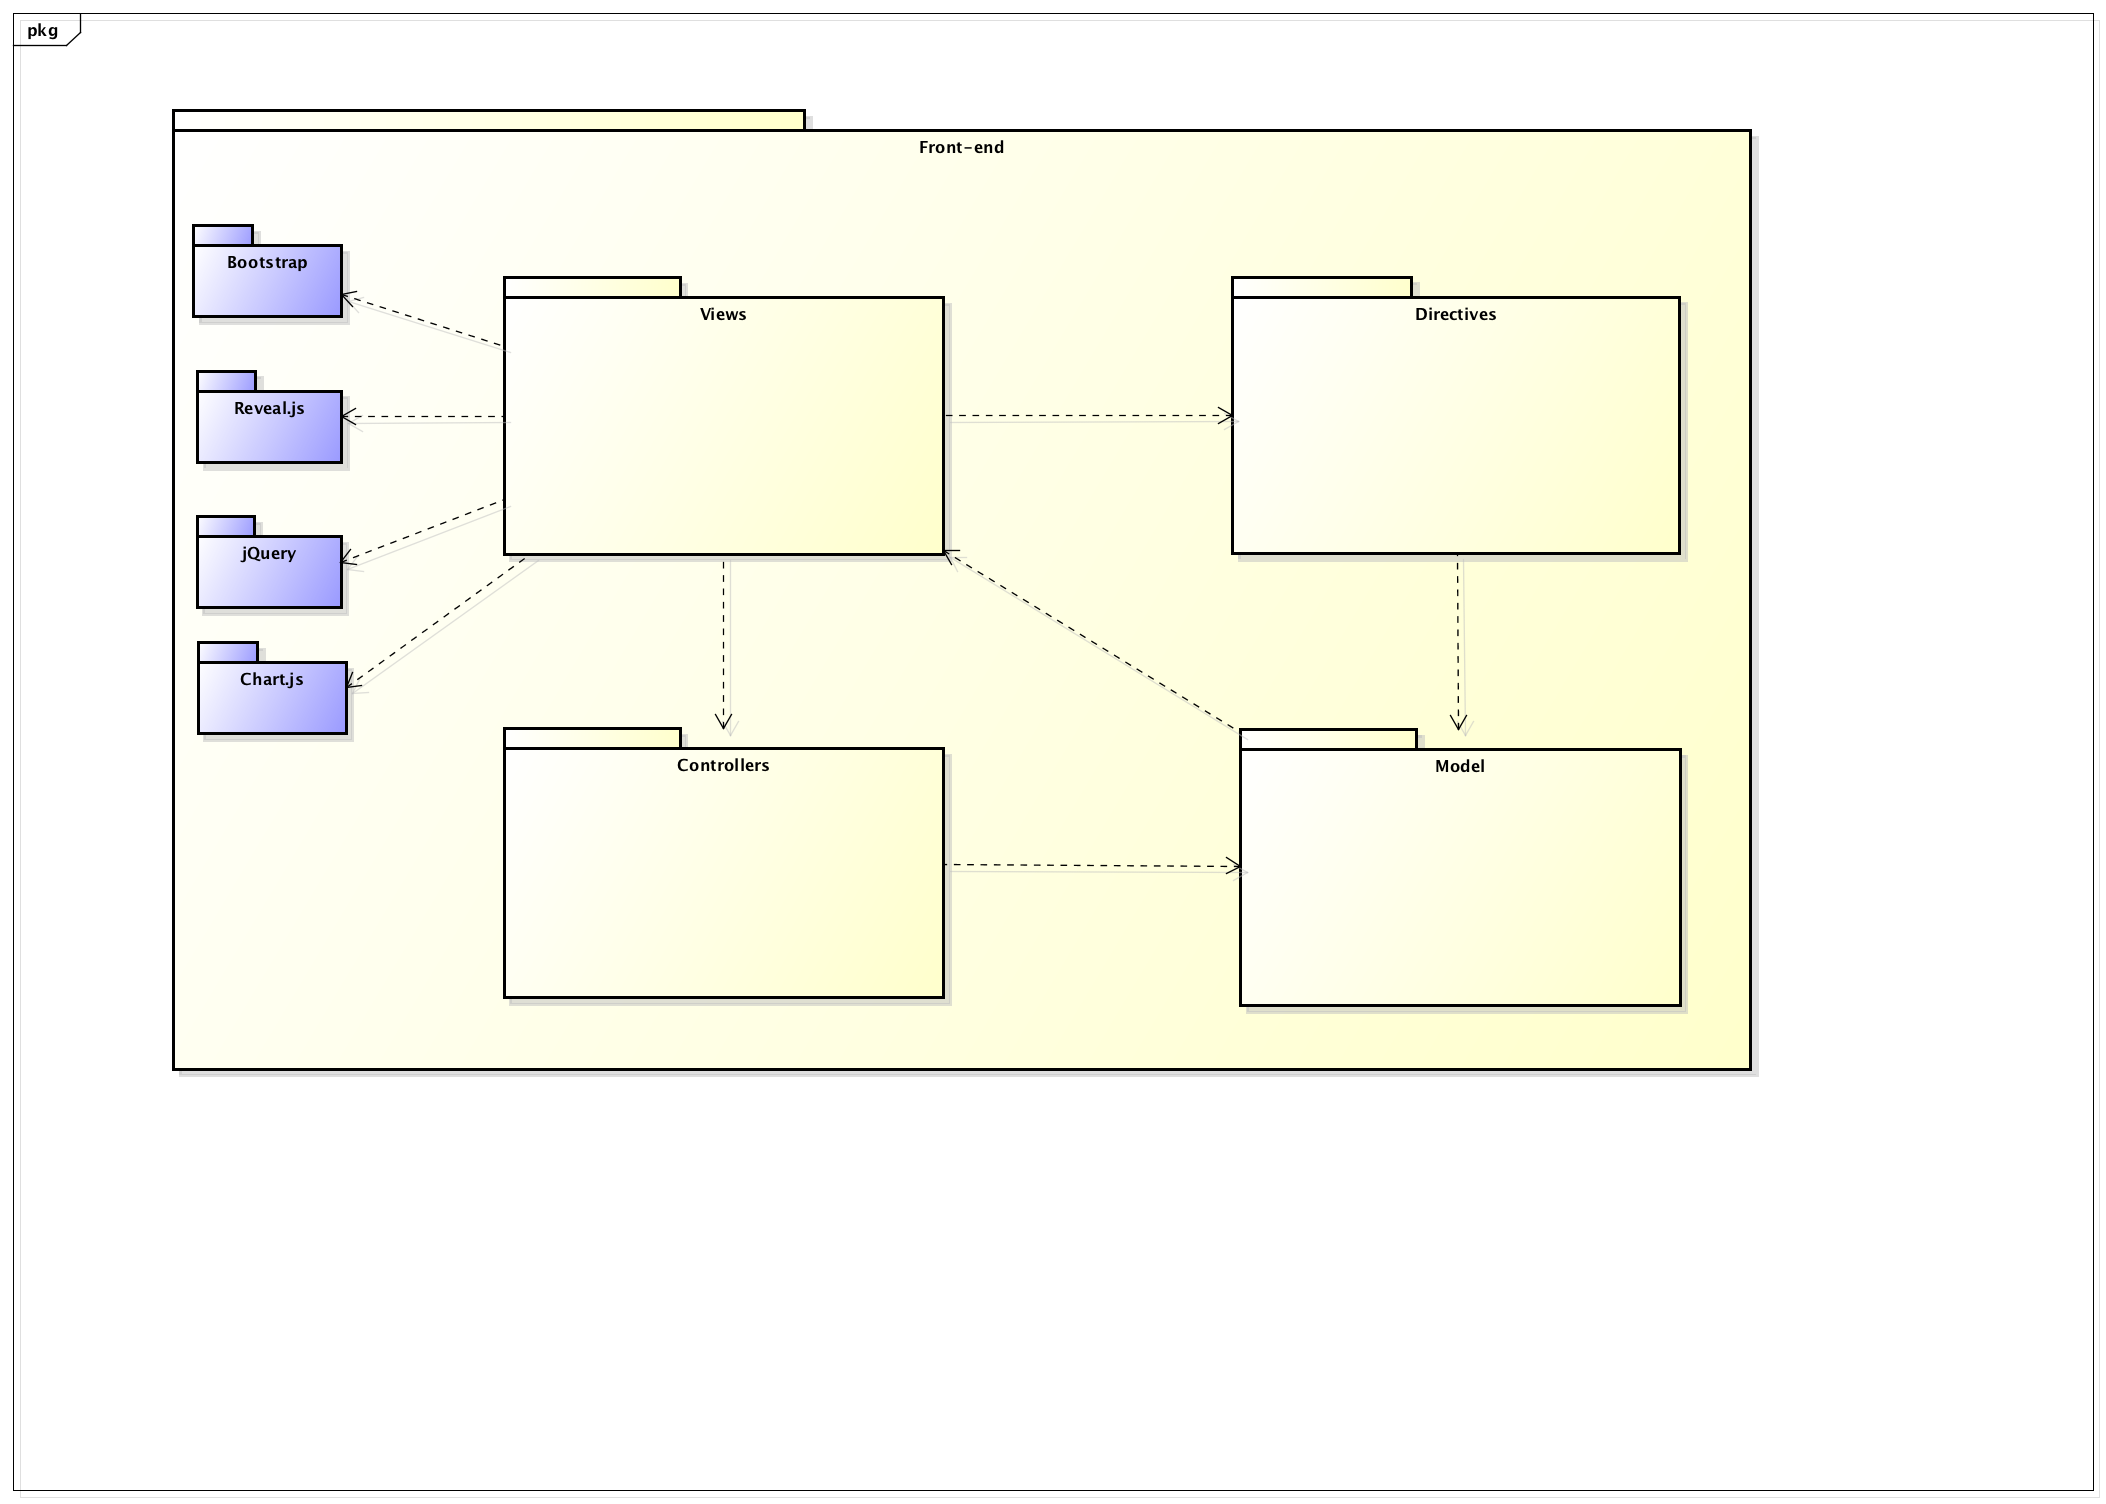
\includegraphics[width=0.9\linewidth]{img/general-front-end}
		\caption[Premi::Front-End]{Premi::Front-End}
		\end{figure}

	Il package contiene i vari componenti della parte di front-end dell'applicazione.
	\\Package contenuti:
	\begin{itemize}
		\item \textbf{View:} Package contenente le views della componente front-end dell'applicazione;
		\item \textbf{Directives:} Package contenente le directives che compongono la view;
		\item \textbf{Model:} Package che definiscono la bussiness logic dell'applicazione;
		\item \textbf{Controller:} Package contenente i controller della parte front-end dell'applicazione.
	\end{itemize}